\documentclass[12pt,a4paper]{article}
\usepackage[utf8]{inputenc}
\usepackage[portuguese]{babel}
\usepackage{graphicx}
\usepackage{subcaption}
\usepackage{geometry}
\usepackage{booktabs}
\usepackage{tabularx}
\usepackage{hyperref}
\usepackage{cite}
\usepackage{float}
\usepackage{longtable}
\usepackage{array}
\usepackage{indentfirst}
\usepackage{tabularx}
\usepackage[table]{xcolor}
\usepackage{makecell}
\usepackage{fontawesome5}
\usepackage{todonotes}
\newcolumntype{Y}{>{\raggedright\arraybackslash}X}
\newcounter{epico}
\newcounter{historia}

\geometry{a4paper, margin=2cm}

\title{\textbf{Atividade 3 - Elicitação e Requisitos}\\
\large MC656 - Engenharia de Software}
\author{
  Caio Lima Albuquerque - RA: 288808 \\
  Giovana Jacome Marchetti - RA: 177700 \\
  Julia de Souza Nardo - RA: 281272 \\
  Leonardo Carvalho De Luca - RA: 288820\\
  Samuel Rodrigues Ferreira - RA: 195440
}
\date{\today}

\begin{document}

\maketitle

\section{Introdução}
Este documento reúne o registro da elicitação de requisitos do projeto, a análise que
transformou as descobertas em requisitos, os épicos e histórias resultantes e a
priorização do \textit{backlog}. O código já existente (Atividade 2) não foi interrompido: os requisitos aqui descritos orientam e refinam o trabalho que continua em andamento.

O fluxo seguido pela equipe foi:

\begin{center}
\small
Elicitação (entrevistas e \textit{brainstorming}) $\rightarrow$ Descobertas $\rightarrow$ Análise $\rightarrow$
Requisitos funcionais e não funcionais $\rightarrow$ Épicos $\rightarrow$ Histórias
$\rightarrow$ Critérios de aceitação $\rightarrow$ Backlog priorizado
\end{center}

\textbf{Onde estão os artefatos no GitHub:} todas as issues desta atividade possuem a label \texttt{Atividade3}; as histórias referenciam o épico correspondente por \texttt{\#N} e o backlog está organizado no GitHub Projects do grupo:

\begin{center}
    \href{https://github.com/users/GiizAzul/projects/1}\faGithub\texttt{ https://github.com/users/GiizAzul/projects/1}
\end{center}

\begin{figure}[h]
\centering 
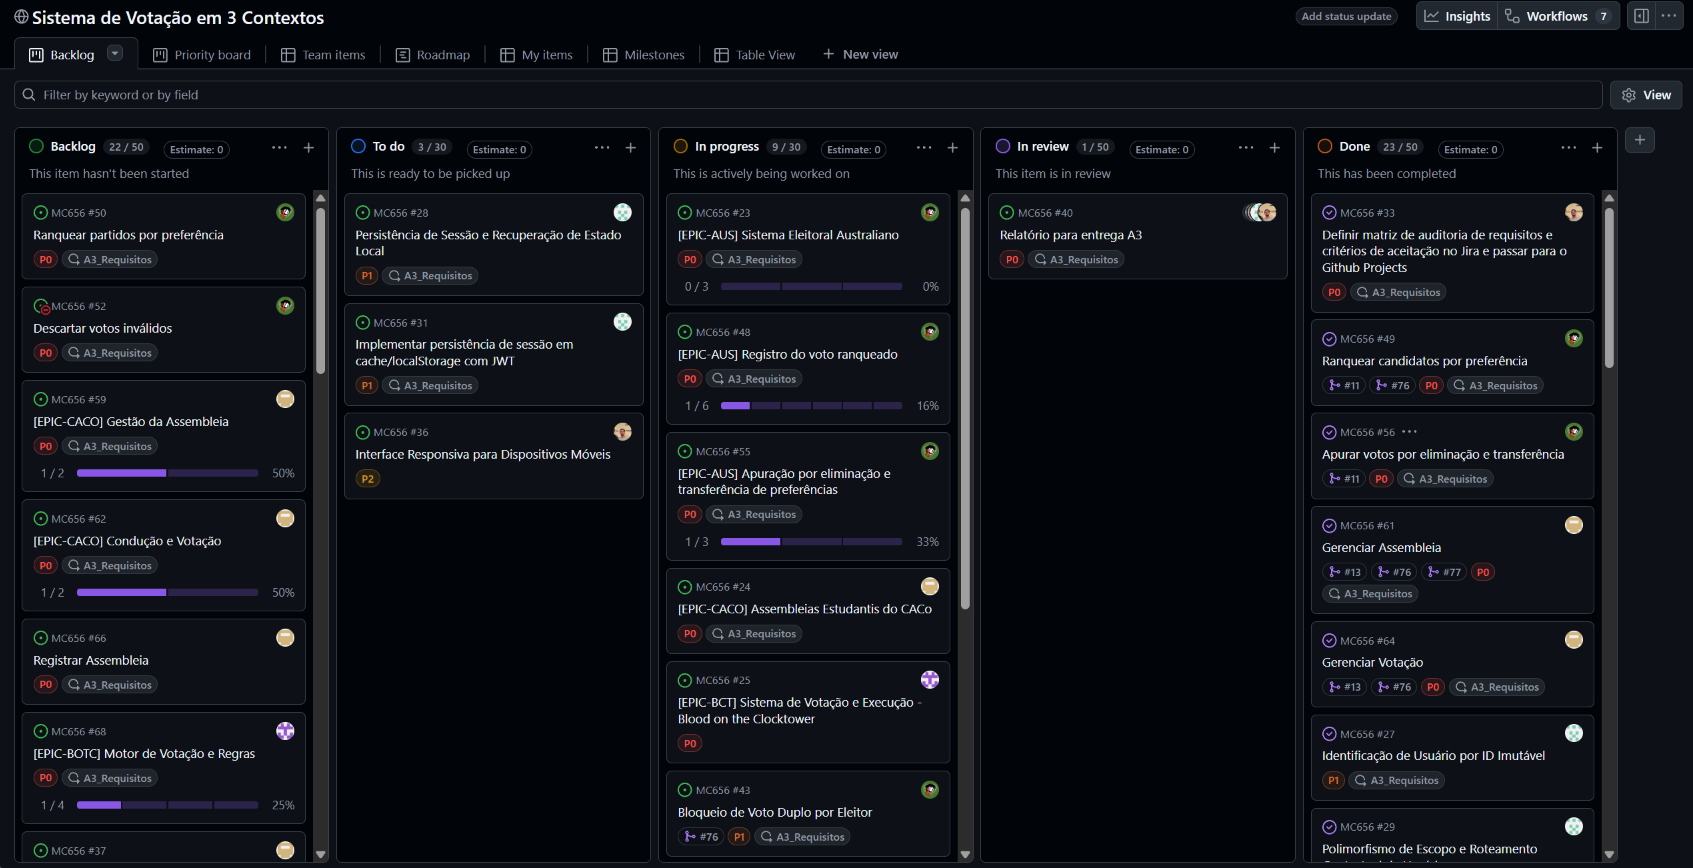
\includegraphics[width=0.7\textwidth]{imagens/ilustracao_project.png} 
\caption{Registro da organização e priorização do \textit{Projects}} 
\label{fig:ilustracao_project}
\end{figure}

\newpage

\section{Elicitação de requisitos}

\subsection{Técnica escolhida e justificativa}

As técnicas utilizadas foram a \textbf{entrevista semiestruturada} e o \textbf{brainstorming}. 

A \textbf{entrevista semiestruturada} foi aplicada nos três contextos do sistema, permitindo que a equipe compreendesse as regras de negócio complexas de cada domínio eleitoral (Austrália, BotC e CACo) diretamente com usuários familiarizados com essas dinâmicas. 

Complementarmente, a equipe realizou sessões de \textbf{brainstorming} interno para levantar e alinhar os requisitos transversais da aplicação, focando principalmente nas necessidades arquiteturais de autenticação e segurança, além da usabilidade e transição da interface de terminal (CLI) para uma interface gráfica Web.

\subsection{Participantes e fontes}

Abaixo seguem informações sobre os participantes das entrevistas:
\begin{table}[H]
\centering
\small
\begin{tabular}{c m{10cm} c m{8cm}}
\toprule
\textbf{Contexto} & \textbf{Perfil} & \textbf{Modo / Duração} \\
\hline

Austrália &
Cidadão australiano com vivência com eleições australianas, como eleitor e voluntário, além de ter votado tanto no país quanto no exterior &
Online / 31 min 56 s \\
\hline

BotC & 
Jogador há 1.5 anos com experiência presencial e online (site oficial BotC online). Já atuou como Mestre (Storyteller) em partidas. & 
Presencial / 20 min 49 s \\
\hline
CACo & Estudante de Ciência da Computação na Unicamp e atual membro da Gestão do CACo & Presencial / 24 min 14 s
\\


\bottomrule
\end{tabular}
\caption{Fontes utilizadas na elicitação.}
\end{table}

\subsection{Evidências}

Para demonstrar a execução efetiva do processo de elicitação, registramos as evidências de ambas as técnicas utilizadas. Para as \textbf{entrevistas semiestruturadas} (realizadas nos três contextos), disponibilizamos os roteiros, gravações em áudio e transcrições, que pode ser acessado através do link abaixo: 

\begin{center}
\href{https://drive.google.com/drive/folders/1s8ZZ3xeoJ77NYrVhzbvqrNzkEsC5gDiC?usp=sharing}{
    
\includegraphics[height=1em]{imagens/google-drive.png}
    \,Evidências do processo de elicitação de requisitos}
\end{center}

Além disso, o \textbf{brainstorming} do grupo veio principalmente de uma reunião do grupo realizada online no por meio do Google Meet no dia 6 de setembro:

\begin{center}
\href{https://docs.google.com/spreadsheets/d/1ETcw3FcnQh86l495lMvo9exbDIIsuBCawLOc9AhvOtc/edit?usp=sharing}{
    
\includegraphics[height=1em]{imagens/sheets.png}
    \,Relatório de participação em reunião do grupo no dia 6 de setembro}
\end{center}

Elaboramos também um quadro síntese das discussões internas da equipe, como se observa na tabela abaixo:

\begin{table}[H]
    \centering
    \small
    \renewcommand{\arraystretch}{1.5}
    \begin{tabular}{|m{3.5cm}|m{6.5cm}|m{5cm}|}
        \hline
        \rowcolor[gray]{0.9}
        \textbf{Foco de Discussão} & \textbf{Ideias Levantadas} & \textbf{Requisito relacionado} \\
        \hline
        
        \textbf{Interface Gráfica} & 
        O grupo discutiu que a votação precisa ser acessível e prática, priorizando uma interface web simples no lugar de comandos de texto. & 
        Abandono do CLI (utilizada para prototipação). Adoção de arquitetura Web com formulários e botões via navegador. \\
        \hline

        \textbf{Responsividade (Mobile)} & 
        O grupo discutiu que usuários participarão das assembleias e jogos presencialmente, utilizando majoritariamente a tela do celular. & 
        Interface adaptativa (design responsivo), evitando quebra horizontal em listas e botões com área de toque adequada para smartphones. \\
        \hline
        
        \textbf{Segurança e Identidade} & 
        O grupo discutiu que é necessário evitar colisões de identificadores e fraudes na identificação dos usuários. & 
        Implementação de UUID v4 invisível ao usuário como chave primária real. \textit{Username} ou RA passam a ser apenas formas de acesso. \\
        \hline

        \textbf{Roteamento e Controle de Acesso} & 
        O grupo discutiu que, existindo 3 sistemas no mesmo domínio, o usuário se perderia facilmente se precisasse escolher seu contexto manualmente. & 
        Polimorfismo de escopo (RBAC). Redirecionamento automático pós-login para o contexto correto e bloqueio (HTTP 403) de URLs não autorizadas. \\
        \hline
        
        \textbf{Sessão e Conectividade} & 
        O grupo discutiu que o sistema deve manter o estado da sessão mesmo diante de quedas de conexão ou atualizações da página. & 
        Implementação de persistência de estado local (Cookies HTTPOnly / Local Storage) para manter o usuário logado e no contexto correto. \\
        \hline

        \textbf{Fluxo de Múltiplas Votações} & 
       O grupo discutiu que assembleias possuem pautas sequenciais, e exigir login a cada nova votação geraria muita frustração. & 
        Manutenção do token ativo e criação de um \textit{Dashboard} central para retorno automático após cada confirmação de voto. \\
        \hline
        
    \end{tabular}
    \caption{Quadro síntese do \textit{brainstorming} da equipe de desenvolvimento sobre requisitos transversais.}
    \label{tab:brainstorming}
\end{table}

\clearpage
\section{Da elicita\c{c}\~ao aos requisitos}

\subsection{Rastreabilidade: descoberta $\rightarrow$ an\'alise $\rightarrow$ requisito}

%Cada linha relaciona uma descoberta \`a interpreta\c{c}\~ao feita pela equipe e ao requisito (funcional ou n\~ao funcional) e aos itens do backlog que o implementam. Todo \'epico e toda hist\'oria deste documento deve aparecer ao menos uma vez nesta se\c{c}\~ao.

\subsubsection{Eleição no modelo da Austrália}

\begin{longtable}{|p{7cm}|p{4.5cm}|p{4.5cm}|}
    \hline
    \rowcolor[gray]{0.9}
    \textbf{Descoberta da elicitação} &
    \textbf{Análise/Interpretação} &
    \textbf{Requisito relacionado} \\
    \hline

    O entrevistado explica que a eleição da Austrália funciona por meio de ranqueamento das opções (AUS-03)
    & O sistema precisa implementar a votação por ranqueamento.
    & RF: Voto ranqueado
    \newline \newline Épico \#\ref{epico:ranqueamento} \\
    
    \hline
    
    O entrevistado explica que a cédula tem duas formas de preenchimento: ``acima da linha" (numerar os partidos) e "abaixo da linha" (numerar individualmente todos os candidatos) (AUS-03)
    & O sistema precisa oferecer as duas formas de votação.
    & RF: Ranquear candidatos
    \newline \newline História \#\ref{historia:ranqueamento_candidatos}
    \newline \newline
    RF: Ranquear partidos
    \newline \newline História \#\ref{historia:ranqueamento_partidos} \\
    
    \hline
    
    O entrevistado disse que na modalidade ``acima da linha", se o eleitor não numerar todas as preferências, é o próprio partido quem decide o destino dos votos restantes (AUS-03)
    & O sistema deve permitir os partidos elencarem suas prioridades de destino de voto.
    & RF: Partidos escolhem destinos de votos dados a eles
    \newline \newline História \#\ref{historia:ranqueamento_destino} \\
    
    \hline
    
    O entrevistado explicou que votos em branco e com erro de numeração (``voto do burro") são totalmente descartados (AUS-04)
    & O sistema precisa descartar votos com ranking incompleto ou mal numerado.
    & RF: Descarte de votos inválidos
    \newline \newline História \#\ref{historia:ranqueamento_invalido} \\
    
    \hline
    
    Partidos distribuem cartões de instrução de voto fora dos locais de votação; a Comissão Eleitoral apoia pessoas com dificuldade (AUS-05)
    & Como não há voluntários físicos para ajudar o eleitor no sistema, essa orientação precisa estar embutida na própria interface.
    & RF: instruções de votação
    \newline \newline História \#\ref{historia:ranqueamento_orientacao} \\

    \hline
    
    O entrevistado explicou como os nomes dos candidados aparecem nas cédulas, seguido pelo nome do partido (AUS-12)
    & O sistema deve seguir as recomendações de formatação dos nomes dos candidados que o entrevistado informou em AUS-12.
    & RNF: formatação dos nomes dos candidatos
    \newline \newline História \#\ref{historia:ranqueamento_formatacao} \\

    \hline
    
    O entrevistado explicou que dificilmente um candidato vence só com a primeira preferência; a apuração normalmente exige várias rodadas de eliminação e transferência (última eleição citado: vencedor com ~34–35\% de 1ª preferência) (AUS-11)
    & Confirma que o algoritmo de apuração precisa implementar eliminação e redistribuição iterativa como caminho normal, não exceção
    & RF: Apuração por eliminação e transferência
    \newline \newline Épico \#\ref{epico:apuracao} \\
    
    \hline
    
    O entrevistado elucidou que a apuração é pública: resultados provisórios são liberados progressivamente conforme os votos são contados, e qualquer pessoa pode observar o processo (AUS-08)
    & O sistema deve expor o andamento da apuração enquanto ela ocorre, não só o resultado final, mantendo a transparência observada no processo real.
    & RF: exibir contagem parcial por candidato durante a apuração
    \newline \newline História \#\ref{historia:apuracao_parcial} \\
    
    \hline

    Pedido direto do entrevistado: gostaria de ver um gráfico mostrando a redistribuição de votos entre os dois candidatos com mais votos, rodada a rodada, até alguém passar de 50\% (AUS-16)
    & Necessidade explícita de visualização da evolução da apuração — citada pelo próprio entrevistado como a principal melhoria desejada.
    & RNF: visualização do resultado de forma constante
    \newline \newline  História \#\ref{historia:apuracao_visualizacao} \\

    \hline
    
    O entrevistado explicou que a identidade do eleitor é checada por nome (sem exigir documento) contra o registro do distrito; pergunta-se se já votou em outro lugar, criando obrigação legal de não votar duas vezes (AUS-10)
    & Equivale ao que o épico transversal de autenticação já deve cobrir; reforça a necessidade de impedir voto duplicado.
    & RNF: impedir voto duplo
    \newline \newline Transversal ao Épico \#\ref{epico:autenticacao} \\
    \hline
    \caption{Rastreabilidade do contexto Austrália.}
\end{longtable}


\subsubsection{Blood on the Clocktower}

\begin{longtable}{|p{7cm}|p{4.5cm}|p{4.5cm}|}
    \hline
    \rowcolor[gray]{0.9}
    \textbf{Descoberta da elicitação} &
    \textbf{Análise/Interpretação} &
    \textbf{Requisito relacionado} \\
    \hline

    O entrevistado explicou que para ir à forca, o jogador precisa de mais de 50\% dos votos vivos. Para substituir alguém na forca, precisa ultrapassar os votos do anterior. Em caso de empate, ambos saem da forca (BOT-08).
    & A regra de cálculo para a execução não é uma maioria simples; o sistema deve rastrear o ocupante atual da forca e aplicar regras estritas de substituição e anulação por empate.
    & RF: Cálculo de Veredito e Substituição na Forca
    \newline \newline Épico \#\ref{epico:botc_execucao} 
    \newline História \#\ref{historia:botc_veredito} \\
    
    \hline
    
    O entrevistado apontou que a maior confusão na contagem ocorre quando habilidades alteram o peso dos votos (ex: voto vale por 3 ou votos negativados) (BOT-09).
    & A contagem automatizada não pode assumir que cada jogador contribui com "1" voto. O sistema deve suportar modificadores matemáticos associados a jogadores específicos.
    & RF: Suporte a modificadores de peso de voto
    \newline \newline História \#\ref{historia:botc_modificadores} \\
    
    \hline
    
    Os votos dos mortos são vitais para o balanceamento (impedem vitória fácil do mal). Um jogador morto possui exatamente um "voto fantasma" pelo resto do jogo, acompanhado no jogo físico por uma vela (BOT-10).
    & O sistema precisa distinguir o status do jogador (vivo/morto), permitir o uso de um único voto pós-morte e bloquear interações de votação subsequentes desse jogador.
    & RF: Controle de elegibilidade e Voto Fantasma
    \newline \newline História \#\ref{historia:botc_status} \\
    
    \hline
    
    O entrevistado avisou que permitir a consulta de quem votou em quem (histórico aberto) a qualquer momento desbalanceia o jogo, pois entrega deduções sociais prontas para o time do bem (BOT-06).
    & O sistema não pode possuir logs abertos de votos acessíveis aos jogadores. A transparência dos votos deve ser efêmera (apenas visualizada no momento em que ocorrem).
    & RNF: Ocultação de histórico de votos na partida
    \newline \newline História \#\ref{historia:botc_ocultacao} \\

    \hline
    
    O maior pedido do entrevistado ("fallback") foi para lidar com quedas de internet de quem estiver usando o celular para votar, o que forçaria o mestre a refazer a contagem (BOT-13, BOT-18).
    & A infraestrutura deve persistir a intenção de voto do cliente e o andamento da contagem no backend para tolerar desconexões e recarregamento da página sem perder dados.
    & RNF: Persistência de sessão e resiliência
    \newline \newline Transversal ao Épico \#\ref{epico:autenticacao} \\
    \hline
    \caption{Rastreabilidade do contexto do BotC.}
\end{longtable}

\subsubsection{Assembleia do CACo}

\begin{longtable}{|p{7cm}|p{4.5cm}|p{4.5cm}|}
    \hline
    \rowcolor[gray]{0.9}
    \textbf{Descoberta da elicitação} & \textbf{Análise/Interpretação} & \textbf{Requisito relacionado} \\
    \hline
    A assinatura presencial é díficil de manejar durante a assembléia e gera filas muito grandes (CAC-13) & 
    
    A presença deve ser registrada de maneira mais eficiente, permitindo cadastros durante toda o período anterior à votação. 
    
    & RF: Registro de presença 
    \newline \newline  História \#\ref{historia:gerenciar_assembleia}\\
    
    \hline
    O entrevistado explica que nome e RA são utilizados para confirmar a identidade (CAC-12) 
    
    & O sistema precisa de controle de acesso baseado em atributos, barrando votos de usuários não presentes na lista oficial.
    
    & RF: Verificação de elegibilidade
    \newline \newline História \#\ref{historia:gerenciar_assembleia}\\
    
    \hline
    O quórum estatutário relatado é de 10\% dos alunos de graduação. Se não for atingido no início, a assembleia vira uma "plenária" sem poder deliberativo (CAC-06, CAC-07)
    
    & O sistema deve calcular o quórum em tempo real e bloquear tecnicamente a abertura de votações se o mínimo não for atingido.
    
    & RF: Cálculo automático do quórum   
    \newline \newline História \#\ref{historia:gerenciar_assembleia}\\
    
    \hline
    O entrevistado afirma que podem ocorrer múltiplas votações em uma mesma assembleia (CAC-08)
    
    &A quantidade de ciclos de votação é variável 
    
    & RF: Gerenciamento de ciclos
    \newline \newline Épico \#\ref{epico:votacao}\\
    \hline
    O entrevistado aponta que a divulgação de votos vinculados ao nome do votante ou da contagem em tempo real podem influenciar a escolha dos participantes (CAC-11, CAC-14)
    
    &Deve-se prezar pelo anonimato dos votantes e confiabilidade dos resultados 
    
    &RNF: Anonimato e confiabilidade
    \newline \newline História \#\ref{historia:gerenciar_votacao}\\
    \hline
     O método de apuração atual consiste de uma análise de contraste visual, podendo ser substituida por uma contagem manual mediante consentimento dos votantes (CAC-04)
     
     &O sistema deve otimizar o registro/ apuração dos votos, desvinculando da necessidade de contagem visual ou manual. 
     
     & RF: Contagem e apuração de votos
     \newline \newline Épico \#\ref{epico:votacao}\\
    \hline
    A condução da assembleia é responsabilidade de uma pessoa específica (CAC-08) 
    
    &Deve existir um papel de responsável pela condução.
    
    &RF: Cadastro de pautas e opções de votação/ Controle da abertura e encerramento
    \newline \newline Épico \#\ref{epico:gestao}\\
    \hline
    O método visual de garantia de voto único é sujeito a erros (CAC-05)
    
    &O sistema deve garantir voto único.
    
    &RF: Voto único 
    \newline \newline História \#\ref{historia:gerenciar_votacao}\\
    \hline
    A ata é pública e registra falas e resultado após o fim da assembleia e ela pode melhorar a acessibilidade para pessoas que chegam atrasadas ou não conseguem acompanhar/escutar a assembleia (CAC-10, CAC-13)
    
    &Deve ser possível acessar de modo facilitado a ata a longo prazo. 
    
    &RF: Registro do histórico
    \newline \newline História \#\ref{historia:registrar_assembleia}
    \newline \newline RF: Acessibilidade da ata
    \newline \newline História\#\ref{historia:consultar_ata}\\
    \hline
    O entrevistado apontou dificuldades no controle e ordenação das falas (CAC-13)
    
    &Deve existir uma fila estruturada de inscrições para fala. 
    
    & RF: Gerenciamento da fila de fala 
    \newline \newline História \#\ref{historia:gerenciar_falas}\\
    \hline
    O entrevistado considera útil saber quantas pessoas conseguiriam comparecer (CAC-15) 
    
    &Pode haver uma funcionalidade de confirmação/intenção de participação. 
    
    &RF: Manifestação de intenção 
    \newline \newline Épico \#\ref{epico:registro}\\
    \hline
    \caption{Rastreabilidade do contexto do CACo}
\end{longtable}

\subsubsection{Requisitos Transversais (Autenticação e Interface Web)}

\begin{longtable}{|p{7cm}|p{4.5cm}|p{4.5cm}|}
    \hline
    \rowcolor[gray]{0.9}
    \textbf{Descoberta da elicitação} & \textbf{Análise/Interpretação} & \textbf{Requisito relacionado} \\
    \hline
    
    A equipe de desenvolvimento identificou que utilizar o \textit{username} como chave primária deixava o sistema vulnerável a colisões de nomes e fraudes de personificação (Brainstorming Interno). 
    & A identidade do usuário no banco de dados deve ser desvinculada do nome de exibição, exigindo a adoção de identificadores únicos (UUID v4) gerados pelo backend para manter a integridade dos votos.
    & RF: Identificação Unívoca por ID Imutável
    \newline \newline História \#\ref{historia:auth_id}
    \newline \newline Épico \#\ref{epico:autenticacao} \\
    
    \hline
    
    A equipe notou que, existindo múltiplos sistemas eleitorais integrados, o usuário poderia acessar painéis incorretos ou se perder ao navegar manualmente (Brainstorming Interno).
    & O sistema deve identificar o escopo (perfil) do usuário no momento do login e roteá-lo automaticamente, bloqueando acessos a áreas não autorizadas (HTTP 403).
    & RF: Roteamento Contextual e Controle de Acesso
    \newline \newline História \#\ref{historia:auth_polimorfismo} 
    \newline \newline Épico \#\ref{epico:autenticacao} \\

    \hline
    
    A equipe manifestou preocupação com a perda de progresso durante as votações devido a quedas de internet ou recarregamento acidental da página (Brainstorming Interno).
    & O sistema não pode tratar cada requisição de forma isolada; é necessário manter um token salvo de forma segura no cliente para restaurar o estado da sessão automaticamente.
    & RNF: Persistência de Sessão e Recuperação de Estado Local
    \newline \newline História \#\ref{historia:auth_sessao} 
    \newline \newline Épico \#\ref{epico:autenticacao} \\
    
    \hline
    
    A equipe relatOu que a utilização de um terminal de comandos (CLI) impunha uma alta barreira de entrada, inviabilizando o uso por eleitores e jogadores comuns (Brainstorming Interno).
    & A aplicação precisa ser migrada para uma plataforma acessível, onde o fluxo inteiro (login, navegação e voto) ocorra por meio de cliques visuais e não por digitação de comandos.
    & RNF: Interação Intuitiva e Usabilidade (Interface Web)
    \newline \newline História \#\ref{historia:web_ui} 
    \newline \newline Épico \#\ref{epico:interface_web} \\

    \hline

    Foi levantado que usuários participarão das assembleias e jogos presencialmente, utilizando majoritariamente a tela do celular (Brainstorming Interno).
    & A interface web precisa ser responsiva, adaptando botões para a área de toque (touch) e evitando quebras de layout horizontal em telas menores.
    & RNF: Interface Responsiva para Dispositivos Móveis
    \newline \newline História \#\ref{historia:web_mobile} 
    \newline \newline Épico \#\ref{epico:interface_web} \\
    
    \hline

    Assembleias costumam ter várias pautas sequenciais. Exigir um novo login a cada votação geraria atrito e lentidão no processo (Brainstorming Interno).
    & O sistema deve possuir um painel central (\textit{Dashboard}) que mantenha a sessão ativa e permita retornar à lista de votações instantaneamente após confirmar um voto.
    & RF: Fluxo de Múltiplas Votações na Mesma Sessão
    \newline \newline História \#\ref{historia:web_multi_voto} 
    \newline \newline Épico \#\ref{epico:interface_web} \\

    \hline
    \caption{Rastreabilidade dos requisitos transversais (Autenticação e Interface).}
\end{longtable}

\section{\'Epicos, hist\'orias e crit\'erios de aceita\c{c}\~ao}

\subsection{Vis\~ao geral}

\begin{table}[H]
    \centering
    \begin{tabular}{|c|p{7cm}|c|p{4.5cm}|}
    \hline
    \rowcolor[gray]{0.9}
    \textbf{Issue} & \textbf{Épico} & \textbf{Contexto} & \textbf{Histórias} \\
    \hline
    
    \href{https://github.com/GiizAzul/MC656/issues/48}{\#48} & \ref{epico:ranqueamento}. Registro do voto ranqueado & Austrália & \#\ref{historia:ranqueamento_candidatos}, \#\ref{historia:ranqueamento_partidos}, \#\ref{historia:ranqueamento_destino}, \#\ref{historia:ranqueamento_invalido}, \#\ref{historia:ranqueamento_orientacao}, \#\ref{historia:ranqueamento_formatacao} \\
    
    \href{https://github.com/GiizAzul/MC656/issues/55}{\#55} & \ref{epico:apuracao}. Apuração por eliminação e transferência de preferências & Austrália & \#\ref{historia:apuracao_eliminacao}, \#\ref{historia:apuracao_parcial}, \#\ref{historia:apuracao_visualizacao} \\

    \href{https://github.com/GiizAzul/MC656/issues/68}{\#68} & \ref{epico:botc_execucao}. Motor de Votação e Regras & BotC & \#\ref{historia:botc_veredito}, \#\ref{historia:botc_modificadores}, \#\ref{historia:botc_status}, \#\ref{historia:botc_ocultacao} \\
    
    \href{https://github.com/GiizAzul/MC656/issues/26}{\#26} & \ref{epico:autenticacao}. Arquitetura de Autenticação e Sessão Multi-Escopo & Transversal & \#\ref{historia:auth_id}, \#\ref{historia:auth_sessao}, \#\ref{historia:auth_polimorfismo} \\

    \href{https://github.com/GiizAzul/MC656/issues/34}{\#34} & \ref{epico:interface_web}. Interface Gráfica e Usabilidade Web & Transversal & \#\ref{historia:web_ui}, \#\ref{historia:web_mobile}, \#\ref{historia:web_multi_voto}\\
    
    \href{https://github.com/GiizAzul/MC656/issues/59}{\#59} & \ref{epico:gestao}. Gestão da Assembleia & CACo & \#\ref{historia:consultar_assembleia}, \#\ref{historia:gerenciar_assembleia}\\
    
    \href{https://github.com/GiizAzul/MC656/issues/62}{\#62} & \ref{epico:votacao}. Condução e votação & CACo & \#\ref{historia:gerenciar_falas}, \#\ref{historia:gerenciar_votacao}\\
    
    \href{https://github.com/GiizAzul/MC656/issues/65}{\#65} & \ref{epico:registro}. Registro e transparência & CACo & \#\ref{historia:registrar_assembleia}, \#\ref{historia:consultar_ata}\\
    
    \hline
    \end{tabular}
    \caption{Épicos e histórias.}
\end{table}

\refstepcounter{epico}
\label{epico:ranqueamento}
\subsection*{Épico \ref{epico:ranqueamento} --- Registro do voto ranqueado (Austrália)}

\renewcommand{\arraystretch}{1.5}
\begin{table}[H]
    \centering
    \begin{tabular}{|m{4.5cm} | m{11cm}|}
    \hline
    
    \textbf{Propósito e valor} &
    Permitir que o eleitor expresse sua preferência completa entre os candidatos, reproduzindo o modelo de voto preferencial australiano, e garantir que o voto só seja aceito quando preenchido corretamente. \\
    
    \textbf{Origem} &
    AUS-03, AUS-04, AUS-05, AUS-12 \\
    
    \textbf{Escopo} &
    Inclui: interface de ranqueamento (1 a N), validação de preenchimento completo e sem repetições, orientações de preenchimento, cadastro de candidatos com nome completo e partido. \\
    
    
    \textbf{Situação atual no código} &
    Avançado --- A coleta da cédula via Web foi implementada com validações matemáticas estritas no backend: o sistema barra completamente e avisa o eleitor caso ele envie uma cédula com menos opções que o exigido, com posições repetidas (empates) ou numeração pulada (ex: 1, 3, 4). Também já foi implementada a trava de "voto único" que impede submissões duplicadas. Ainda sem orientação ao eleitor sobre partidos e dados melhores descritos. \\    
    \hline
    \end{tabular}
\end{table}

\vspace{0.5cm}

\refstepcounter{historia}
\label{historia:ranqueamento_candidatos}
\begin{table}[H]
    \centering
    \begin{tabular}{|m{4.5cm} | m{11cm}|}
    \hline
    
    \multicolumn{2}{|l|}{\textbf{História \#\ref{historia:ranqueamento_candidatos} --- Ranquear candidatos por preferência}} \\
    
    \hline   \textbf{História} &
    \textbf{Como} eleitor, \newline
    \textbf{quero} ranquear todos os candidatos por ordem de preferência, \newline  
    \textbf{para} expressar minha escolha completa conforme o modelo de voto preferencial australiano. \\
    
    \textbf{Critérios de aceitação} &
    \begin{itemize}
        \item{Verificar se o sistema apresenta a lista de candidatos (nome completo e partido) para atribuição de posição de 1 a N.}
        \item{Verificar se o sistema impede o envio enquanto houver candidatos sem posição ou posições repetidas.}
        \item{Verificar se, ao tentar enviar um ranking inválido, o sistema informa quais posições faltam ou estão repetidas.}
    \end{itemize}\\
    
    
    \textbf{Origem} &
    AUS-03 \\
    
    \textbf{Depende de} &
    --- \\
    
    \hline
    \end{tabular}
\end{table}

\refstepcounter{historia}
\label{historia:ranqueamento_partidos}
\begin{table}[H]
    \centering
    \begin{tabular}{|m{4.5cm} | m{11cm}|}
    \hline
    
    \multicolumn{2}{|l|}{\textbf{História \#\ref{historia:ranqueamento_partidos} --- Ranquear partidos por preferência}} \\
    
    \hline  \textbf{História} &
    \textbf{Como} eleitor, \newline
    \textbf{quero} poder ranquear os partidos por ordem de preferência, \newline  
    \textbf{para} votar de forma mais rápida e simples. \\
    
    \textbf{Critérios de aceitação} &
    \begin{itemize}
        \item{Verificar se o sistema apresenta a lista de partidos para atribuição de posição de 1 a N.}
        \item{Verificar se o sistema impede o envio enquanto houver partidos sem posição ou posições repetidas.}
        \item{Verificar se, ao tentar enviar um ranking inválido, o sistema informa quais posições faltam ou estão repetidas.}
    \end{itemize}\\
    
    
    \textbf{Origem} &
    AUS-03 \\
    
    \textbf{Depende de} &
    --- \\
    
    \hline
    \end{tabular}
\end{table}

\refstepcounter{historia}
\label{historia:ranqueamento_destino}
\begin{table}[H]
    \centering
    \begin{tabular}{|m{4.5cm} | m{11cm}|}
    \hline
    
    \multicolumn{2}{|l|}{\textbf{História \#\ref{historia:ranqueamento_destino} --- Partido pode alocar aos seus candidatos votos destinados a ele}} \\
    
    \hline  \textbf{História} &
    \textbf{Como} partido, \newline
    \textbf{quero} distribuir livremente os votos que foram dados a mim aos meus candidatos, \newline  
    \textbf{para} tomar a ação que favorece a minha eleição. \\
    
 \textbf{Critérios de aceitação} &
    \begin{itemize}
        \item{Verificar se o sistema permite ao partido definir uma ordem de preferência entre seus candidatos.}
        \item{Verificar se o sistema utiliza a ordem definida pelo partido para distribuir os votos destinados a ele quando o eleitor votar acima da linha.}
    \end{itemize}\\

    
    
    \textbf{Origem} &
    AUS-03 \\
    
    \textbf{Depende de} &
    História \#\ref{historia:ranqueamento_partidos} \\
    
    \hline
    \end{tabular}
\end{table}

\refstepcounter{historia}
\label{historia:ranqueamento_invalido}
\begin{table}[H]
    \centering
    \begin{tabular}{|m{4.5cm} | m{11cm}|}
    \hline
    
    \multicolumn{2}{|l|}{\textbf{História \#\ref{historia:ranqueamento_invalido} --- Descartar votos inválidos}} \\
    
    \hline  \textbf{História} &
    \textbf{Como} partido, \newline
    \textbf{quero} que os votos em branco ou com erro de numeração sejam descartados da contagem, \newline  
    \textbf{para} que o resultado da eleição não seja distorcido por votos inválidos. \\
    
    \textbf{Critérios de aceitação} &
    \begin{itemize}
        \item{Verificar se o sistema classifica como inválido votos completamente em branco, com numeração incompleta ou repetida.}
        \item{Verificar se um voto classificado como inválido é excluído da apuração.}
        \item{Verificar se o sistema registra a quantidade de votos descartados por tipo de invalidade para consulta pós-eleição}
    \end{itemize}\\
    
    
    \textbf{Origem} &
    AUS-04 \\
    
    \textbf{Depende de} &
    Histórias \#\ref{historia:ranqueamento_candidatos} ou \#\ref{historia:ranqueamento_partidos} \\
    
    \hline
    \end{tabular}
\end{table}

\refstepcounter{historia}
\label{historia:ranqueamento_orientacao}
\begin{table}[H]
    \centering
    \begin{tabular}{|m{4.5cm} | m{11cm}|}
    \hline
    
    \multicolumn{2}{|l|}{\textbf{História \#\ref{historia:ranqueamento_orientacao} --- Orientar o preenchimento do voto}} \\
    
    \hline  \textbf{História} &
    \textbf{Como} eleitor com dificuldade, \newline
    \textbf{quero} ver instruções de como preencher corretamente meu ranking antes de votar, \newline  
    \textbf{para} reduzir a chance de meu voto ser descartado por erro de preenchimento. \\
    
    \textbf{Critérios de aceitação} &
    \begin{itemize}
        \item{Verificar se o sistema exibe explicação de como votar e do que é um voto válido.}
        \item{Verificar se, em envio inválido, mostra o motivo específico (ex.: "faltam 2 candidatos sem posição").}
    \end{itemize}\\
    
    
    \textbf{Origem} &
    AUS-05 \\
    
    \textbf{Depende de} &
    --- \\
    
    \hline
    \end{tabular}
\end{table}

\refstepcounter{historia}
\label{historia:ranqueamento_formatacao}
\begin{table}[H]
    \centering
    \begin{tabular}{|m{4.5cm}|m{11cm}|}
    \hline

    \multicolumn{2}{|l|}{
        \textbf{História \#\ref{historia:ranqueamento_formatacao} --- Formatação dos nomes dos candidatos}
    } \\

    \hline

    \textbf{História} &
    \textbf{Como} eleitor,
    \newline
    \textbf{quero} ler e conseguir diferenciar claramente os candidatos disponíveis,
    \newline
    \textbf{para} conseguir votar sem nenhuma dúvida e necessidade de desambiguação na hora da votação. \\

    \textbf{Critérios de aceitação} &
    \begin{itemize}
        \item{Verificar se o sistema apresenta o candidato no formato: SOBRENOME, Nome, Partido.}
        \item{Verificar se, quando necessário para diferenciar candidatos, o sistema apresenta informações adicionais do nome, como o nome do meio.}
    \end{itemize}\\
    
    \textbf{Origem} &
    AUS-12 \\

    \textbf{Depende de} &
    História \#\ref{historia:ranqueamento_candidatos} \\

    \hline
    \end{tabular}
\end{table}

\refstepcounter{epico}
\label{epico:apuracao}
\subsection*{Épico \ref{epico:apuracao} --- Apuração por eliminação e transferência de preferências (Austrália)}

\renewcommand{\arraystretch}{1.5}
\begin{table}[H]
    \centering
    \begin{tabular}{|m{4.5cm} | m{11cm}|}
    \hline
    
    \textbf{Propósito e valor} &
    Reproduzir a apuração por rodadas do voto preferencial australiano, eliminando o candidato com menos votos e redistribuindo suas preferências até haver um vencedor com maioria, além de tornar esse processo transparente. \\
    
    \textbf{Origem} &
    AUS-07, AUS-08, AUS-11, AUS-16 \\
    
    \textbf{Escopo} &
    Inclui: algoritmo iterativo de eliminação/transferência, exibição de resultados parciais, visualização da evolução entre os dois principais candidatos. \\
    
    
    \textbf{Situação atual no código} &
    Parcial --— há fluxo básico de votação via terminal, sem validação de ranking completo nem orientação ao eleitor. \\
    
    \hline
    \end{tabular}
\end{table}

\refstepcounter{historia}
\label{historia:apuracao_eliminacao}
\begin{table}[H]
    \centering
    \begin{tabular}{|m{4.5cm}|m{11cm}|}
    \hline

    \multicolumn{2}{|l|}{
        \textbf{História \#\ref{historia:apuracao_eliminacao} --- Apurar votos por eliminação e transferência}
    } \\

    \hline

    \textbf{História} &
    \textbf{Como} sistema eleitoral,
    \newline
    \textbf{quero} eliminar candidatos e redistribuir suas preferências a cada rodada,
    \newline
    \textbf{para} realizar a apuração conforme o modelo de voto preferencial australiano. \\

    \textbf{Critérios de aceitação} &
    \begin{itemize}
        \item{Verificar se o sistema identifica o candidato com menor quantidade de votos em cada rodada.}
        \item{Verificar se os votos do candidato eliminado são redistribuídos conforme as preferências seguintes.}
        \item{Verificar se o sistema repete as rodadas de eliminação e transferência até que haja um vencedor com maioria.}
    \end{itemize}\\

    \textbf{Origem} &
    AUS-11 \\

    \textbf{Depende de} &
    Histórias \#\ref{historia:ranqueamento_candidatos} e \#\ref{historia:ranqueamento_partidos} \\

    \hline
    \end{tabular}
\end{table}

\refstepcounter{historia}
\label{historia:apuracao_parcial}
\begin{table}[H]
    \centering
    \begin{tabular}{|m{4.5cm} | m{11cm}|}
    \hline
    
    \multicolumn{2}{|l|}{\textbf{História \#\ref{historia:apuracao_parcial} --- Exibir contagem parcial por candidato durante a apuração}} \\
    
    \hline \textbf{História} &
    \textbf{Como} eleitor,
    \newline
    \textbf{quero} acompanhar a contagem dos votos durante a apuração,
    \newline
    \textbf{para} observar o andamento da eleição antes do resultado final. \\
    
    \textbf{Critérios de aceitação} &
    \begin{itemize}
        \item{Verificar se o sistema exibe os resultados parciais conforme os votos são contabilizados.}
        \item{Verificar se o sistema permite acompanhar a quantidade de votos de cada candidato durante a apuração.}
        \item{Verificar se os resultados parciais são atualizados ao longo das rodadas de apuração.}
    \end{itemize}\\
    
    \textbf{Origem} &
    AUS-08 \\
    
    \textbf{Depende de} &
    Histórias \#\ref{historia:ranqueamento_candidatos} e \#\ref{historia:ranqueamento_partidos} \\
    
    \hline
    \end{tabular}
\end{table}

\refstepcounter{historia}
\label{historia:apuracao_visualizacao}
\begin{table}[H]
    \centering
    \begin{tabular}{|m{4.5cm}|m{11cm}|}
    \hline

    \multicolumn{2}{|l|}{
        \textbf{História \#\ref{historia:apuracao_visualizacao} --- Visualizar a evolução da apuração}
    } \\

    \hline

    \textbf{História} &
    \textbf{Como} eleitor,
    \newline
    \textbf{quero} visualizar graficamente a redistribuição dos votos durante a apuração,
    \newline
    \textbf{para} acompanhar a evolução do resultado rodada a rodada. \\

    \textbf{Critérios de aceitação} &
    \begin{itemize}
        \item{Verificar se o sistema apresenta graficamente a quantidade de votos dos candidatos ao longo das rodadas.}
        \item{Verificar se o sistema permite visualizar a redistribuição dos votos após a eliminação de um candidato.}
        \item{Verificar se a visualização acompanha a evolução da apuração até que um candidato ultrapasse 50\% dos votos.}
    \end{itemize}\\

    \textbf{Origem} &
    AUS-16 \\

    \textbf{Depende de} &
    História \#\ref{historia:apuracao_eliminacao} \\

    \hline
    \end{tabular}
\end{table}

\vspace{0.5cm}

\vspace{0.5cm}

\refstepcounter{epico}
\label{epico:botc_execucao}
\subsection*{Épico \ref{epico:botc_execucao} --- Motor de Votação e Regras (BotC)}

\renewcommand{\arraystretch}{1.5}
\begin{table}[H]
    \centering
    \begin{tabular}{|m{4.5cm} | m{11cm}|}
    \hline
    \textbf{Propósito e valor} &
    Automatizar a contagem matemática complexa, as regras de substituição de forca e o uso de votos fantasmas, aliviando a carga cognitiva do Mestre e mitigando erros de esquecimento de modificadores. \\
    \textbf{Origem} & Entrevistas BotC (BOT-06 a BOT-10, BOT-13 e BOT-18). \\
    \textbf{Escopo} & Controle de status de jogadores (vivo/morto), registro de consumo de voto fantasma, aplicação de pesos variáveis aos votos, cálculo de empate e substituição na forca, e restrição de acesso a histórico. \\
    \textbf{Situação atual no código} & Parcial --— Há lógica de votação genérica e uma interface restrita do Storyteller criada e testada na Web, garantindo que usuários com papel de "Jogador" comum sejam barrados via erro 403 (Acesso Negado) se tentarem forjar o registro de uma execução ou apuração de votos. A distinção de status de vida e a não execução de ninguém em caso de empate já estão parcialmente implementadas, ainda deve ser escalada para ficar com a lógica perfeita. Ainda não há limitadores de voto fantasma nem mecânicas de mudança nos pesos dos votos ou possibilidades de votos serem impedidos por habilidades no jogo. \\
    \hline
    \end{tabular}
\end{table}

\vspace{0.5cm}

\refstepcounter{historia}
\label{historia:botc_veredito}
\begin{table}[H]
    \centering
    \begin{tabular}{|m{4.5cm} | m{11cm}|}
    \hline
    \multicolumn{2}{|l|}{\textbf{História \#\ref{historia:botc_veredito} --- Determinação do Veredito da Forca}} \\
    \hline  \textbf{História} &
    \textbf{Como} Mestre (Storyteller), \newline
    \textbf{quero} que o sistema aplique as regras de desempate e maioria dinamicamente, \newline  
    \textbf{para} determinar automaticamente se o nomeado atual vai para a forca, substitui o jogador anterior, ou se ambos se salvam em caso de empate. \\
    \textbf{Critérios de aceitação} &
    \begin{itemize}
        \item{O sistema deve calcular mais de 50\% dos vivos como requisito base inicial.}
        \item{Se já houver alguém na forca, a nova contagem deve superar o valor do jogador anterior para substituí-lo.}
        \item{Se a nova contagem empatar com o jogador na forca, o sistema deve remover ambos da forca.}
    \end{itemize}\\
    \textbf{Origem} & BOT-08 \\
    \textbf{Depende de} & --- \\
    \hline
    \end{tabular}
\end{table}

\refstepcounter{historia}
\label{historia:botc_modificadores}
\begin{table}[H]
    \centering
    \begin{tabular}{|m{4.5cm} | m{11cm}|}
    \hline
    \multicolumn{2}{|l|}{\textbf{História \#\ref{historia:botc_modificadores} --- Aplicação de Modificadores de Voto}} \\
    \hline  \textbf{História} &
    \textbf{Como} Mestre (Storyteller), \newline
    \textbf{quero} poder atribuir pesos diferentes aos votos de jogadores específicos (ex: valer por 3, ou negativo), \newline  
    \textbf{para} que habilidades de classes afetem o veredito sem gerar erros de cálculo humano. \\
    \textbf{Critérios de aceitação} &
    \begin{itemize}
        \item{O sistema deve permitir que o Mestre configure modificadores ocultos em jogadores antes ou durante as votações.}
        \item{Ao apurar os votos, o sistema deve multiplicar ou reduzir matematicamente o total com base nos modificadores.}
    \end{itemize}\\
    \textbf{Origem} & BOT-09 \\
    \textbf{Depende de} & História \#\ref{historia:botc_veredito} \\
    \hline
    \end{tabular}
\end{table}

\refstepcounter{historia}
\label{historia:botc_status}
\begin{table}[H]
    \centering
    \begin{tabular}{|m{4.5cm} | m{11cm}|}
    \hline
    \multicolumn{2}{|l|}{\textbf{História \#\ref{historia:botc_status} --- Controle de Status e Voto Fantasma}} \\
    \hline  \textbf{História} &
    \textbf{Como} Jogador de BotC, \newline
    \textbf{quero} que o sistema controle meu status de vida e registre se eu possuo meu voto fantasma, \newline  
    \textbf{para} que o balanceamento da partida seja mantido e votos mortos extras não sejam computados por acidente. \\
    \textbf{Critérios de aceitação} &
    \begin{itemize}
        \item{O sistema exibe o status atual do jogador na interface (Vivo, Morto com Voto, Morto sem Voto).}
        \item{O sistema computa o voto de um jogador "Morto" e imediatamente remove o seu privilégio de voto fantasma para as próximas rodadas.}
        \item{Bloquear a UI de votação para mortos que já gastaram o fantasma.}
    \end{itemize}\\
    \textbf{Origem} & BOT-10 \\
    \textbf{Depende de} & --- \\
    \hline
    \end{tabular}
\end{table}

\refstepcounter{historia}
\label{historia:botc_ocultacao}
\begin{table}[H]
    \centering
    \begin{tabular}{|m{4.5cm} | m{11cm}|}
    \hline
    \multicolumn{2}{|l|}{\textbf{História \#\ref{historia:botc_ocultacao} --- Ocultação do Histórico de Votos na Partida}} \\
    \hline  \textbf{História} &
    \textbf{Como} Jogador do time do Mal, \newline
    \textbf{quero} que o histórico detalhado de quem votou em quem não fique visível para consulta posterior durante a partida, \newline  
    \textbf{para} que o time do Bem não utilize o sistema como uma ferramenta artificial para descobrir alinhamentos de forma facilitada. \\
    \textbf{Critérios de aceitação} &
    \begin{itemize}
        \item{A interface dos jogadores nunca exibe log ou histórico das rodadas anteriores de votação.}
        \item{Apenas o resultado numérico final da forca daquela nomeação é persistido visivelmente; a autoria dos votos deve sumir da UI após o encerramento da contagem.}
    \end{itemize}\\
    \textbf{Origem} & BOT-06 \\
    \textbf{Depende de} & --- \\
    \hline
    \end{tabular}
\end{table}


\refstepcounter{epico}
\label{epico:autenticacao}
\subsection*{Épico \ref{epico:autenticacao} --- Arquitetura de Autenticação e Sessão Multi-Escopo (Transversal)}

\renewcommand{\arraystretch}{1.5}
\begin{table}[H]
    \centering
    \begin{tabular}{|m{4.5cm} | m{11cm}|}
    \hline
    
    \textbf{Propósito e valor} &
    Criar um método de verificação utilizando chaves primárias imutáveis (como UUID) e manter a persistência de sessão e roteamento multi-contexto, garantindo que a identidade do eleitor/jogador seja única e persistente e evitando perda de votos por queda de conexão. \\
    
    \textbf{Origem} & Brainstorming Interno \\
    
    \textbf{Escopo} &
    Inclui: geração de identificadores únicos (UUID v4), refatoração do código para referenciar estritamente o User\_ID, armazenamento seguro de token de sessão no cliente, recuperação de estado após fechamento da página e roteamento automático de contexto. \\
    
    \textbf{Situação atual no código} &
    Implementado --- O sistema agora gera e rastreia o User\_ID imutável, permitindo o login tanto via \textit{Username} quanto via RA (para estudantes do CACo). A persistência de sessão foi implementada utilizando Cookies HTTP (httponly), garantindo que o usuário seja redirecionado automaticamente e não perca o estado de autenticação entre diferentes votações, além de travas rígidas de escopo que impedem o acesso cruzado entre domínios. \\
    
    \hline
    \end{tabular}
\end{table}

\vspace{0.5cm}

\refstepcounter{historia}
\label{historia:auth_id}
\begin{table}[H]
    \centering
    \begin{tabular}{|m{4.5cm} | m{11cm}|}
    \hline
    
    \multicolumn{2}{|l|}{\textbf{História \#\ref{historia:auth_id} --- Identificação de Usuário por ID Imutável}} \\
    
    \hline  \textbf{História} &
    \textbf{Como} Desenvolvedor e Administrador de Segurança, \newline
    \textbf{quero} que o sistema gere e utilize um ID único (ex: UUID v4) como chave primária interna para todas as transações, votos e auditorias, \newline  
    \textbf{para} garantir a integridade dos dados, prevenir fraudes de personificação e permitir que o username seja apenas um atributo de exibição. \\
    
    \textbf{Critérios de aceitação} &
    \begin{itemize}
        \item{Toda nova conta criada deve receber um identificador único alfanumérico/numérico imutável gerado pelo backend.}
        \item{Todas as tabelas/estruturas de log de voto, presença em assembleia e sessões de jogo devem referenciar exclusivamente o User\_ID, nunca o username.}
        \item{O sistema deve impedir colisões de identidade mesmo que dois contextos utilizem nomes de exibição semelhantes.}
        \item{Tentativas de forjar votos alterando nomes de exibição na camada de apresentação devem ser completamente inócuas para o banco de dados.}
    \end{itemize}\\
    
    \textbf{Origem} &
    Brainstorming Interno \\
    
    \textbf{Depende de} &
    --- \\
    \hline
    \end{tabular}
\end{table}

\refstepcounter{historia}
\label{historia:auth_sessao}
\begin{table}[H]
    \centering
    \begin{tabular}{|m{4.5cm} | m{11cm}|}
    \hline
    
    \multicolumn{2}{|l|}{\textbf{História \#\ref{historia:auth_sessao} --- Persistência de Sessão e Recuperação de Estado Local}} \\
    
    \hline  \textbf{História} &
    \textbf{Como} Usuário do Sistema de Votação (Jogador, Estudante ou Eleitor), \newline
    \textbf{quero} que minha sessão permaneça salva localmente em cache/storage seguro após o login, \newline  
    \textbf{para} não precisar redigitar credenciais caso feche a aba, recarregue a página ou ocorra uma oscilação na conexão. \\
    
    \textbf{Critérios de aceitação} &
    \begin{itemize}
        \item{Após o login bem-sucedido, o token de autenticação/sessão deve ser armazenado de forma segura no cliente.}
        \item{Ao reabrir a aplicação, o sistema deve verificar a validade do token local e restaurar a sessão ativa sem redirecionar para a tela de login.}
        \item{Caso a sessão expire (após TTL configurado) ou o usuário selecione Sair, o cache local de autenticação deve ser limpo imediatamente.}
        \item{O fechamento e reabertura da janela durante uma votação em andamento deve restaurar o usuário diretamente na tela da cédula correspondente.}
    \end{itemize}\\
    
    \textbf{Origem} &
    Brainstorming Interno \\
    
    \textbf{Depende de} &
    História \#\ref{historia:web_ui} e História \#\ref{historia:web_multi_voto}\\
    
    \hline
    \end{tabular}
\end{table}

\vspace{0.5cm}

\refstepcounter{historia}
\label{historia:auth_polimorfismo}
\begin{table}[H]
    \centering
    \begin{tabular}{|m{4.5cm} | m{11cm}|}
    \hline
    
    \multicolumn{2}{|l|}{\textbf{História \#\ref{historia:auth_polimorfismo} --- Polimorfismo de Escopo e Roteamento Contextual de Usuários
}} \\
    
    \hline  \textbf{História} &
    \textbf{Como} Usuário cadastrado em um contexto específico, \newline
    \textbf{quero} ser direcionado automaticamente para o painel correspondente ao meu perfil (Eleitor Austrália, Jogador BCT ou Estudante CACo) logo após o login, \newline  
    \textbf{para} acessar diretamente as funcionalidades relevantes sem navegar por menus desnecessários ou contextos não autorizados. \\
    
    \textbf{Critérios de aceitação} &
    \begin{itemize}
        \item{A entidade de usuário deve conter a definição do seu escopo de autorização (SCOPE\_BCT, SCOPE\_CACO, SCOPE\_AUSTRALIA ou SCOPE\_GLOBAL).}
        \item{O fluxo de login deve inspecionar as permissões do usuário autenticado e despachar a rota inicial adequada.}
        \item{Se um usuário tentar acessar uma rota fora do seu escopo por URL direta, o sistema deve apresentar tela de Acesso Não Autorizado (HTTP 403) e retornar ao seu contexto nativo.}
    \end{itemize}\\
    
    \textbf{Origem} &
    Brainstorming Interno \\
    
    \textbf{Depende de} &
    --- \\
    
    \hline
    \end{tabular}
\end{table}

\vspace{0.5cm}

\refstepcounter{epico}
\label{epico:interface_web}
\subsection*{Épico \ref{epico:interface_web} --- Interface Gráfica e Usabilidade Web (Transversal)}
\renewcommand{\arraystretch}{1.5}
\begin{table}[H]
    \centering
    \begin{tabular}{|m{4.5cm} | m{11cm}|}
    \hline
    \textbf{Propósito e valor} &
    Cumprir o RNF de Usabilidade, substituindo o terminal (CLI) por uma interface gráfica intuitiva e responsiva (podendo escalar para uso mobile). \\
    \textbf{Origem} & Brainstorming Interno \\
    \textbf{Escopo}& Inclui: estruturação do \textit{design system} e desenvolvimento de componentes visuais  para substituir o uso de terminal (CLI) em todos os módulos da aplicação.\\
    \textbf{Situação atual no código}& Implementado. A transição do CLI para a interface Web foi totalmente concluída utilizando FastAPI e Jinja2. Todo o roteamento e a renderização de formulários dinâmicos, dashboards e restrições visuais (botões que só aparecem para a Gestão) estão funcionais, validados e com 100\% de cobertura de testes automatizados nos roteadores. Ainda falta escalar de acordo com as futuras alterações no \textit{backend} e uma estilização aprimorada.\\
    \hline
    \end{tabular}
\end{table}

\refstepcounter{historia}
\label{historia:web_ui}
\begin{table}[H]
    \centering
    \begin{tabular}{|m{4.5cm} | m{11cm}|}
    \hline
    \multicolumn{2}{|l|}{\textbf{História \#\ref{historia:web_ui} --- Interação Intuitiva via Web}} \\
    \hline  \textbf{História} &
    \textbf{Como} usuário sem conhecimento técnico (Eleitor, Jogador ou Estudante), \newline
    \textbf{quero} interagir com o sistema de votação inteiramente através de um navegador web, utilizando botões, menus visuais e formulários,\newline  
    \textbf{para} para que eu não precise aprender, memorizar ou digitar comandos de terminal (CLI) para participar das sessões. \\
    \textbf{Critérios de aceitação} &
    \begin{itemize}
        \item{O usuário deve conseguir realizar todo o fluxo (login, seleção de contexto, votação e logout) através de cliques em uma interface visual no browser.}
        \item{O sistema deve exibir mensagens de feedback visual (ex: toasts de sucesso, modais de erro) no lugar de \textit{prints} no console.}
        \item{A interface não deve exigir que o usuário digite nenhum comando de texto para navegar entre as telas.}
    \end{itemize}\\
    \textbf{Origem}& Brainstorming Interno\\
    \textbf{Depende de}& --- \\
    \hline
    \end{tabular}
\end{table}

\refstepcounter{historia}
\label{historia:web_mobile}
\begin{table}[H]
    \centering
    \begin{tabular}{|m{4.5cm} | m{11cm}|}
    \hline
    \multicolumn{2}{|l|}{\textbf{História \#\ref{historia:web_mobile} --- Interface Responsiva para Dispositivos Móveis}} \\
    \hline  \textbf{História} &
    \textbf{Como} usuário mobile do sistema, \newline
    \textbf{quero} poder acessar e utilizar a plataforma de votação através do navegador do meu celular com a interface adaptada,\newline  
    \textbf{para} que eu tenha a flexibilidade de votar durante uma assembleia ou jogar uma partida de BCT confortavelmente de qualquer lugar, sem precisar de um computador. \\
    \textbf{Critérios de aceitação} &
    \begin{itemize}
        \item{O layout das telas principais (Login, Dashboard, Cédula de Votação) deve se adaptar automaticamente a telas de smartphones (design responsivo).}
        \item{Botões de ação principais (como "Confirmar Voto") devem ter área de toque (touch) adequada para polegares.}
        \item{Listas e grids de candidatos/jogadores não devem quebrar horizontalmente, utilizando rolagem ou empilhamento vertical em telas menores.}
    \end{itemize}\\
    \textbf{Origem}& Brainstorming Interno\\
    \textbf{Depende de}& História \#\ref{historia:web_ui} \\
    \hline
    \end{tabular}
\end{table}

\vspace{0.5cm}

\refstepcounter{historia}
\label{historia:web_multi_voto}
\begin{table}[H]
    \centering
    \begin{tabular}{|m{4.5cm} | m{11cm}|}
    \hline
    \multicolumn{2}{|l|}{\textbf{História \#\ref{historia:web_multi_voto} --- Fluxo de Múltiplas Votações na Mesma Sessão}} \\
    \hline  \textbf{História} &
    \textbf{Como} usuário logado no sistema, \newline
    \textbf{quero} poder retornar ao menu principal após concluir um voto e selecionar uma nova eleição ou pauta ativa sem precisar refazer o login,\newline  
    \textbf{para} que eu tenha uma experiência fluida ao participar de sessões com várias votações sequenciais. \\
    \textbf{Critérios de aceitação} &
    \begin{itemize}
        \item{Após confirmar o voto e visualizar o recibo, deve haver um botão claro "Voltar ao Dashboard".}
        \item{Ao clicar em retornar, o sistema deve manter o token do usuário ativo.}
        \item{O Dashboard central deve listar todas as eleições/pautas disponíveis, indicando visualmente quais o usuário já participou (estado concluído) e quais estão pendentes.}
    \end{itemize}\\
    \textbf{Origem}& Brainstorming Interno\\
    \textbf{Depende de}& História \#\ref{historia:web_ui} \\
    \hline
    \end{tabular}
\end{table}

\refstepcounter{epico}
\label{epico:gestao}
\subsection*{Épico \ref{epico:gestao} --- Gestão da Assembleia (CACo)}

\renewcommand{\arraystretch}{1.5}
\begin{table}[H]
    \centering
    \begin{tabular}{|m{4.5cm} | m{11cm}|}
    \hline
    
    \textbf{Propósito e valor} &
    Permitir que o CACo organize uma assembleia, disponibilize suas informações e controle a presença necessária para determinar se ela possui quórum deliberativo. \\
    
    \textbf{Origem} & CAC-05, CAC-06, CAC-08, CAC-12, CAC-13, CAC-15  \\
    
    \textbf{Escopo} &
    Inclui: criação da assembleia, registro de pauta/data, cadastro e identificação dos participantes, verificação de elegibilidade de voto e cálculo do quórum necessário para a realização da assembleia. \\
    
    
    \textbf{Situação atual no código} &
    Parcial --- há implementação de verificação das condições de votação e elegibilidade, porém o processo de registro de presença e cadastro de nova assembleia ainda não contempla todo o fluxo identificado na elicitação. \\
    
    \hline
    \end{tabular}
\end{table}

\vspace{0.5cm}

\refstepcounter{historia}
\label{historia:consultar_assembleia}
\begin{table}[H]
    \centering
    \begin{tabular}{|m{4.5cm} | m{11cm}|}
    \hline
    
    \multicolumn{2}{|l|}{\textbf{História \#\ref{historia:consultar_assembleia} --- Consultar Assembleia}} \\
    
    \hline  \textbf{História} &
    \textbf{Como} aluno de computação, \newline
    \textbf{quero} consultar as assembleias programadas \newline  
    \textbf{para} saber quando elas ocorrerão e qual será sua pauta. \\
    
    \textbf{Critérios de aceitação} &
    \begin{itemize}
        \item{ O sistema deve apresentar as assembleias programadas.}
        \item{Cada assembleia deve apresentar sua data.}
        \item{Cada assembleia deve apresentar sua pauta ou descrição.}
        \item{O participante deve conseguir identificar a assembleia antes de acessá-la.}
    \end{itemize}\\
    
    \textbf{Origem} &
    CAC-05, CAC-15 \\
    
    \textbf{Depende de} &
    História \#\ref{historia:gerenciar_assembleia} \\
    \hline
    \end{tabular}
\end{table}
\refstepcounter{historia}
\label{historia:gerenciar_assembleia}
\begin{table}[H]
    \centering
    \begin{tabular}{|m{4.5cm} | m{11cm}|}
    \hline
    
    \multicolumn{2}{|l|}{\textbf{História \#\ref{historia:gerenciar_assembleia} --- Gerenciar Assembleia}} \\
    
    \hline  \textbf{História} &
    \textbf{Como} condutor, \newline
    \textbf{quero} cadastrar assembleias, registrar presenças e verificar o quórum automaticamente \newline  
    \textbf{para} saber se a assembleia pode ser iniciada. \\
    
    \textbf{Critérios de aceitação} &
    \begin{itemize}
        \item{O sistema deve permitir registro único da presença de um participante mediante sua identificação.}
        \item{O sistema deve verificar se o participante pertence ao grupo elegível para voto.}
        \item{O sistema deve contabilizar os participantes presentes.}
        \item{O sistema deve calcular o quórum de acordo com a quantidade de alunos elegíveis.}
        \item{O sistema deve indicar se o quórum foi atingido.}
    \end{itemize}\\
    
    \textbf{Origem} &
    CAC-13, CAC-12, CAC-06, CAC-08 \\
    
    \textbf{Depende de} &
    --- \\
    
    \hline
    \end{tabular}
\end{table}

\refstepcounter{epico}
\label{epico:votacao}
\subsection*{Épico \ref{epico:votacao} --- Condução e votação (CACo)}

\renewcommand{\arraystretch}{1.5}
\begin{table}[H]
    \centering
    \begin{tabular}{|m{4.5cm} | m{11cm}|}
    \hline
    
    \textbf{Propósito e valor} &
    Permitir a administração de ciclos da assembleia, gerenciamento de inscrições para fala e realização de votações anônimas. \\

    \textbf{Origem} & CAC-04, CAC-05, CAC-08, CAC-13, CAC-14\\
    
    \textbf{Escopo} &
    Inclui: abertura e encerramento de ciclos de votações e deliberação, apresentação das opções de voto, registro de votos, controle de votos duplicados, apuração dos resultados e gerenciamento da ordem de falas. \\
    
    
    \textbf{Situação atual no código} &
    Avançado --- Há implementação da lógica de apuração e contagem de votos e foi implementado o painel de condução exclusivo para a Gestão do CACo, capaz de iniciar e encerrar o ciclo de votação da Assembleia. O sistema possui trava de voto duplo, coleta secreta dos votos e um dashboard de resultados dinâmico que gera barras de progresso proporcionais ao total de votos apurados. A fila de falas e as atas ainda não estão integradas.\\
    \hline
    \end{tabular}
\end{table}

\vspace{0.5cm}

\refstepcounter{historia}
\label{historia:gerenciar_falas}
\begin{table}[H]
    \centering
    \begin{tabular}{|m{4.5cm} | m{11cm}|}
    \hline
    
    \multicolumn{2}{|l|}{\textbf{História \#\ref{historia:gerenciar_falas} --- Gerenciar Falas}} \\
    
    \hline  \textbf{História} &
    \textbf{Como} participante da assembleia, \newline
    \textbf{quero} me inscrever e consultar a ordem de falas \newline  
    \textbf{para} organizar minha participação durante os debates. \\

    \textbf{Critérios de aceitação} &
    \begin{itemize}
        \item{O participante deve poder solicitar inscrição para fala.}
        \item{O sistema deve ordenar as falas, alocando reinscrições após pessoas que ainda não tiveram falas}
        \item{O sistema deve permitir a vizualização da fila}
    \end{itemize}\\
    
    \textbf{Origem} &
    CAC-13\\
    
    \textbf{Depende de} &
     Historia \#\ref{historia:gerenciar_assembleia} \\
    \hline
    \end{tabular}
\end{table}

\refstepcounter{historia}
\label{historia:gerenciar_votacao}
\begin{table}[H]
    \centering
    \begin{tabular}{|m{4.5cm} | m{11cm}|}
    \hline
    
    \multicolumn{2}{|l|}{\textbf{História \#\ref{historia:gerenciar_votacao} --- Gerenciar Votação}} \\
    
    \hline  \textbf{História} &
    \textbf{Como} participante votante da assembleia, \newline
    \textbf{quero} registrar meu voto sem visualizar os votos dos demais participantes durante a votação \newline  
    \textbf{para} expressar minha opinião sem ser influenciado pelo resultado parcial ou pela opinião dos outros. \\
    
    \textbf{Critérios de aceitação} &
    \begin{itemize}
        \item{ O participante deve conseguir selecionar uma das opções disponíveis para a votação.}
        \item{O sistema deve permitir apenas um voto por participante em cada votação.}
        \item{Participantes não elegíveis para voto devem ser impedidos de votar}
        \item{O sistema não deve apresentar o resultado parcial enquanto a votação estiver aberta.}
        \item{O sistema deve impedir que participantes visualizem quem votou em cada opção.}
        \item{Após o encerramento da votação, o sistema deve apresentar a quantidade de votos por opção}
    \end{itemize}\\
    
    \textbf{Origem} &
    CAC-04,CAC-05,CAC-12\\
    
    \textbf{Depende de} &
    Historia \#\ref{historia:gerenciar_assembleia} \\
    
    \hline
    \end{tabular}
\end{table}
\refstepcounter{epico}
\label{epico:registro}
\subsection*{Épico \ref{epico:registro} --- Registro e transparência (CACo)}

\renewcommand{\arraystretch}{1.5}
\begin{table}[H]
    \centering
    \begin{tabular}{|m{4.5cm} | m{11cm}|}
    \hline
    
    \textbf{Propósito e valor} &
    Registrar as informações relevantes da assembleia e disponibilizá-las posteriormente, permitindo acompanhar as decisões tomadas e consultar o histórico das atividades realizadas. \\

    \textbf{Origem} & CAC-10, CAC-13\\
    
    \textbf{Escopo} &
    Inclui: registro das decisões e resultados das votações, registro das manifestações dos participantes e disponibilização das atas durante a assembleia para consulta posterior. \\
    
    
    \textbf{Situação atual no código} &
    Não implementado --- o código atual concentra-se principalmente na lógica de votação e apuração, não contemplando ainda o registro estruturado e a consulta das informações da assembleia. \\
    
    \hline
    \end{tabular}
\end{table}

\vspace{0.5cm}

\refstepcounter{historia}
\label{historia:registrar_assembleia}
\begin{table}[H]
    \centering
    \begin{tabular}{|m{4.5cm} | m{11cm}|}
    \hline
    
    \multicolumn{2}{|l|}{\textbf{História \#\ref{historia:registrar_assembleia} --- Registrar Assembleia}} \\
    
    \hline  \textbf{História} &
    \textbf{Como} responsável pelo registro da assembleia, \newline
    \textbf{quero} registrar as falas, pautas e resultados das votações,\newline  
    \textbf{para} para manter um histórico do que ocorreu durante a assembleia. \\

    \textbf{Critérios de aceitação} &
    \begin{itemize}
        \item{ O sistema deve permitir registrar as informações relevantes da assembleia.}
        \item{O registro deve permanecer associado à assembleia correspondente.}
    \end{itemize}\\
    
    \textbf{Origem} &
    CAC-13\\
    
    \textbf{Depende de} &
     Historia \#\ref{historia:gerenciar_votacao} \\
    \hline
    \end{tabular}
\end{table}

\refstepcounter{historia}
\label{historia:consultar_ata}
\begin{table}[H]
    \centering
    \begin{tabular}{|m{4.5cm} | m{11cm}|}
    \hline
    
    \multicolumn{2}{|l|}{\textbf{História \#\ref{historia:consultar_ata} --- Consultar Ata}} \\
    
    \hline  \textbf{História} &
    \textbf{Como} participante do CACo, \newline
    \textbf{quero} consultar a ata de uma assembleia, \newline  
    \textbf{para} entender o que foi discutido e decidido mesmo que eu não tenha conseguido acompanhar toda a assembleia.\\
    
    \textbf{Critérios de aceitação} &
    \begin{itemize}
        \item{O participante deve conseguir localizar a ata associada a uma assembleia.}
        \item{O sistema deve disponibilizar a ata atualizada.}
        \item{O acesso à ata não deve exigir que o participante tenha participado da assembleia.}
    \end{itemize}\\
    
    \textbf{Origem} &
    CAC-13\\
    
    \textbf{Depende de} &
    Historia \#\ref{historia:registrar_assembleia} \\
    
    \hline
    \end{tabular}
\end{table}
\section{Organiza\c{c}\~ao e prioriza\c{c}\~ao do backlog}

\subsection{Crit\'erios de prioriza\c{c}\~ao adotados}

O backlog \'e orientado a valor. A ordem de prioridade considerou, nesta sequ\^encia:

\begin{enumerate}
  \item \textbf{Valor para o usu\'ario:} a necessidade e qu\~ao grave
  \'e o problema para o usu\'ario. EXEMPLO DAS ENTREVISTAS
  \item \textbf{Depend\^encias:} itens que bloqueiam outros sobem na fila. EXEMPLO DAS ENTREVISTAS
  \item \textbf{Tempo necessário para implementação:} usado como desempate. Itens que podem ser implementados mais rapidamente tem maior prioridade EXEMPLO DAS ENTREVISTAS
\end{enumerate}

\textbf{No GitHub Projects}, a prioridade está organizada nas três categorias P0, P1 e P2, da maior para a menor prioridade, respectivamente.

\subsection{Priorização dos épicos}

\begin{table}[H]
\centering
\small
\begin{tabular}{|c|m{3.4cm}|c|m{6.7cm}|}
\hline
\rowcolor[gray]{0.9}
\textbf{Prior.} &
\textbf{Épico} &
\makecell{\textbf{Incluído na primeira}\\
\textbf{entrega de valor?}} &
\textbf{Justificativa} \\
\hline

P0 & 
\#\ref{epico:ranqueamento} --- Registro do voto ranqueado (Austrália) & 
Sim & 
Base fundamental para capturar a intenção de voto de forma válida (AUS-03, AUS-04). Bloqueia diretamente a etapa de apuração. \\
\hline

P0 & 
\#\ref{epico:apuracao} --- Apuração por eliminação e transferência (Austrália) & 
Sim & 
Motor matemático central que define o vencedor da eleição (AUS-11). Depende da coleta correta dos votos. \\
\hline

P0 & 
\#\ref{epico:botc_execucao} --- Motor de Votação e Regras (BotC) & 
Sim & 
Automatiza a contagem matemática complexa (BOT-09) e as regras da forca (BOT-08), eliminando a carga cognitiva e erros manuais do Mestre. \\
\hline

P1 & 
\#\ref{epico:autenticacao} --- Arquitetura de Autenticação e Sessão & 
Sim & 
Garante a segurança, unicidade de votos e persistência de sessão contra quedas de internet. Base estrutural transversal. \\
\hline

P1 & 
\#\ref{epico:interface_web} --- Interface Gráfica e Usabilidade Web & 
Sim & 
Cumpre o RNF de Usabilidade, viabilizando o acesso por usuários leigos via navegador e substituindo o terminal (CLI). \\
\hline

P0 & 
\#\ref{epico:gestao} --- Gestão da Assembleia (CACo) & 
Sim & 
Alicerce estrutural do domínio. Sem o registro do evento e verificação de quórum (CAC-06), as votações não possuem validade. \\
\hline

P0 & 
\#\ref{epico:votacao} --- Condução e votação (CACo) & 
Sim & 
Entrega o núcleo de valor para os estudantes: deliberação com voto único, seguro e anônimo. Depende da gestão da assembleia. \\
\hline

P2 & 
\#\ref{epico:registro} --- Registro e transparência (CACo) & 
Não & 
Importante para a memória institucional, mas a redação de atas não bloqueia o funcionamento e pode ser feita externamente no MVP. \\
\hline

\end{tabular}
\caption{Priorização dos épicos.}
\end{table}


\subsection{Priorização das histórias por épico}

\subsubsection{\ref{epico:ranqueamento} Registro do voto ranqueado (Austrália)}

\begin{table}[H]
\centering
\small
\begin{tabular}{|c|m{3.4cm}|c|m{6.7cm}|}
\hline
\rowcolor[gray]{0.9}
\textbf{Prior.} &
\textbf{História} &
\makecell{\textbf{Incluído na primeira}\\
\textbf{entrega de valor?}} &
\textbf{Justificativa} \\
\hline

P0 &
\#\ref{historia:ranqueamento_candidatos} --- Ranquear candidatos por preferência &
Sim &
Funcionalidade central da votação e base para as demais validações. \\

\hline
P0 &
\#\ref{historia:ranqueamento_invalido} --- Descartar votos inválidos &
Sim &
Garante a integridade da votação e depende das formas de ranqueamento. Depende de alguma forma de votação implementada.  \\

\hline
P0 &
\#\ref{historia:ranqueamento_partidos} --- Ranquear partidos por preferência &
Sim &
Segunda forma de votação identificada na elicitação. \\

\hline
P1 &
\#\ref{historia:ranqueamento_orientacao} --- Orientar o preenchimento do voto &
Não &
Reduz erros de preenchimento e auxilia o eleitor, mas não é essencial para o funcionamento \\

\hline
P1 &
\#\ref{historia:ranqueamento_formatacao} --- Formatação dos nomes dos candidatos &
Não &
Facilita a identificação dos candidatos, mas não bloqueia a votação. \\

\hline
P2 &
\#\ref{historia:ranqueamento_destino} --- Partido pode alocar aos seus candidatos votos destinados a ele &
Não &
Depende do ranqueamento de partidos e possui regra adicional de distribuição. \\

\hline
\end{tabular}
\caption{Priorização das histórias do épico Registro do voto ranqueado.}
\end{table}

\subsubsection{\ref{epico:apuracao} Apuração por eliminação e transferência de preferências (Austrália)}

\begin{table}[H]
\centering
\small
\begin{tabular}{|c|m{3.4cm}|c|m{6.7cm}|}
\hline
\rowcolor[gray]{0.9}
\textbf{Prior.} &
\textbf{História} &
\makecell{\textbf{Incluído na primeira}\\
\textbf{entrega de valor?}} &
\textbf{Justificativa} \\
\hline

P0 &
\#\ref{historia:apuracao_eliminacao} --- Apurar votos por eliminação e transferência &
Sim &
É a funcionalidade central da apuração e base para as demais histórias. \\

\hline
P1 &
\#\ref{historia:apuracao_parcial} --- Exibir contagem parcial por candidato durante a apuração &
Não &
Garante transparência e depende da apuração. \\

\hline
P2 &
\#\ref{historia:apuracao_visualizacao} --- Visualizar a evolução da apuração &
Não &
Possui valor para o acompanhamento, mas depende dos resultados da apuração. \\

\hline
\end{tabular}
\caption{Priorização das histórias do épico Apuração por eliminação e transferência de preferências.}
\end{table}

\subsubsection{\ref{epico:botc_execucao} Motor de Votação e Regras (BotC)}

\begin{table}[H]
\centering
\small
\begin{tabular}{|c|m{3.4cm}|c|m{6.7cm}|}
\hline
\rowcolor[gray]{0.9}
\textbf{Prior.} &
\textbf{História} &
\makecell{\textbf{Incluído na primeira}\\
\textbf{entrega de valor?}} &
\textbf{Justificativa} \\
\hline

P0 &
\#\ref{historia:botc_veredito} --- Determinação do Veredito da Forca &
Sim &
Core da mecânica de execução do jogo (BOT-08). Sem tratar substituição e empates corretamente, a partida fica inválida. \\
\hline

P0 &
\#\ref{historia:botc_status} --- Controle de Status e Voto Fantasma &
Sim &
Item vital para o balanceamento (BOT-10). Votos de mortos mantêm o jogo vivo; sem esse controle sistêmico ocorrem erros cruciais do mestre. \\
\hline

P1 &
\#\ref{historia:botc_modificadores} --- Aplicação de Modificadores de Voto &
Sim &
Principal fonte de confusão da contagem (BOT-09). Essencial para comportar scripts avançados (classes que valem por 3 ou negativam votos). \\
\hline

P2 &
\#\ref{historia:botc_ocultacao} --- Ocultação do Histórico de Votos na Partida &
Não &
Extremamente importante para o game design (BOT-06), mas no MVP a ausência de um painel de "Histórico" já cumpre esse papel provisoriamente. \\
\hline

\end{tabular}
\caption{Priorização das histórias do épico Motor de Votação e Regras BotC}
\end{table}

\subsubsection{\ref{epico:autenticacao} Arquitetura de Autenticação e Sessão Multi-Escopo (Transversal)}

\begin{table}[H]
\centering
\small
\begin{tabular}{|c|m{3.4cm}|c|m{6.7cm}|}
\hline
\rowcolor[gray]{0.9}
\textbf{Prior.} &
\textbf{História} &
\makecell{\textbf{Incluído na primeira}\\
\textbf{entrega de valor?}} &
\textbf{Justificativa} \\
\hline

P1 &
\#\ref{historia:auth_id} --- Identificação de Usuário por ID Imutável &
 Sim &
 Garante a integridade dos dados e previne fraudes de identidade.
 \\

\hline
P1 &
\#\ref{historia:auth_sessao} --- Persistência de Sessão e Recuperação de Estado Local &
 Sim &
Evita a perda de progresso durante a votação devido a oscilações de conexão, garantindo a confiabilidade do processo.
 \\

\hline
P1 &
\#\ref{historia:auth_polimorfismo} --- Polimorfismo de Escopo e Roteamento Contextual de Usuários &
 Sim &
Garante que o usuário acesse apenas o painel do seu domínio, evitando navegação indevida e falhas de segurança entre contextos.
 \\

\hline

\end{tabular}
\caption{Priorização das histórias do épico Arquitetura de Autenticação e Sessão Multi-Escopo}
\end{table}

\subsubsection{\ref{epico:interface_web} Interface Gráfica e Usabilidade Web (Transversal)}

\begin{table}[H]
\centering
\small
\begin{tabular}{|c|m{3.4cm}|c|m{6.7cm}|}
\hline
\rowcolor[gray]{0.9}
\textbf{Prior.} &
\textbf{História} &
\makecell{\textbf{Incluído na primeira}\\
\textbf{entrega de valor?}} &
\textbf{Justificativa} \\
\hline

P1 &
\#\ref{historia:web_ui} --- Interação Intuitiva via Web &
 Sim & 
 Viabiliza o uso do sistema por usuários, resolvendo a principal barreira técnica do terminal (CLI).
 \\
\hline

P1 &
\#\ref{historia:web_multi_voto} --- Fluxo de Múltiplas Votações na Mesma Sessão &
 Sim & 
 Evita o atrito e a lentidão de exigir um novo login a cada pauta ou rodada, garantindo a fluidez em sessões contínuas.
 \\
\hline

P2 &
\#\ref{historia:web_mobile} --- Interface Responsiva para Dispositivos Móveis &
 Não & 
 Melhoria de usabilidade e ergonomia. A interface web base já permite o acesso, de modo que o refinamento visual específico para telas menores pode ser postergado.
 \\
\hline

\end{tabular}
\caption{Priorização das histórias do épico Interface Gráfica e Usabilidade Web}
\end{table}

\subsubsection{\ref{epico:gestao} Gestão da Assembleia (CACo)}

\begin{table}[H]
\centering
\small
\begin{tabular}{|c|m{3.4cm}|c|m{6.7cm}|}
\hline
\rowcolor[gray]{0.9}
\textbf{Prior.} &
\textbf{História} &
\makecell{\textbf{Incluído na primeira}\\
\textbf{entrega de valor?}} &
\textbf{Justificativa} \\
\hline

P1 &
\#\ref{historia:consultar_assembleia} --- Consultar Assembleia &
Não &
Facilita a organização, mas a divulgação pode ocorrer por canais externos. Depende da criação da assembleia. \\

\hline
P0 &
\#\ref{historia:gerenciar_assembleia} --- Gerenciar Assembleia &
Sim &
Funcionalidade base para criação do evento, registro de presença e cálculo de quórum. \\

\hline

\end{tabular}
\caption{Priorização das histórias do épico Gestão da Assembleia}
\end{table}

\subsubsection{\ref{epico:votacao} Condução e votação (CACo)}

\begin{table}[H]
\centering
\small
\begin{tabular}{|c|m{3.4cm}|c|m{6.7cm}|}
\hline
\rowcolor[gray]{0.9}
\textbf{Prior.} &
\textbf{História} &
\makecell{\textbf{Incluído na primeira}\\
\textbf{entrega de valor?}} &
\textbf{Justificativa} \\
\hline

P2 &
\#\ref{historia:gerenciar_falas} --- Gerenciar Falas &
Não &
Funcionalidade de conveniência. O controle da fila pode ser feito manualmente nesta primeira entrega. \\

\hline
P0 &
\#\ref{historia:gerenciar_votacao} --- Gerenciar Votação &
Sim &
Núcleo central de valor do sistema. Garante a integridade, anonimato e apuração correta da assembleia. \\

\hline

\end{tabular}
\caption{Priorização das histórias do épico Condução e votação}
\end{table}

\subsubsection{\ref{epico:registro} Registro e transparência (CACo)}

\begin{table}[H]
\centering
\small
\begin{tabular}{|c|m{3.4cm}|c|m{6.7cm}|}
\hline
\rowcolor[gray]{0.9}
\textbf{Prior.} &
\textbf{História} &
\makecell{\textbf{Incluído na primeira}\\
\textbf{entrega de valor?}} &
\textbf{Justificativa} \\
\hline

P2 &
\#\ref{historia:registrar_assembleia} --- Registrar Assembleia &
Não &
Importante para o histórico, mas a redação de atas pode ser feita via ferramentas externas no MVP. \\

\hline
P2 &
\#\ref{historia:consultar_ata} --- Consultar Ata &
Não &
Possui valor para transparência, mas depende estritamente do registro interno de atas. \\

\hline

\end{tabular}
\caption{Priorização das histórias do épico Registro e transparência}
\end{table}

\subsection{Primeira entrega de valor}

A primeira entrega de valor (MVP) da aplicação foca em garantir que os fluxos principais de cada um dos três domínios possam ser executados com segurança do início ao fim, operando de forma coesa sob uma nova arquitetura transversal.

Para isso, foram selecionadas todas as histórias de \textbf{Prioridade 0 (P0)} e algumas histórias estruturais de \textbf{Prioridade 1 (P1)}. O conjunto selecionado é coerente pois engloba:

\begin{enumerate}
\item \textbf{A nova arquitetura transversal (P1):} O núcleo de Autenticação com identificadores únicos imutáveis (UUID) e persistência local de sessão, garantindo que não haja vulnerabilidades de personificação, votos duplicados ou perdas de progresso por oscilação de internet.
\item \textbf{A migração para a Interface Web (P1):} A substituição integral do terminal (CLI) por uma interface gráfica intuitiva, viabilizando o uso do sistema por eleitores e jogadores leigos através de navegadores e dispositivos móveis.
\item \textbf{No contexto Austrália (P0):} O registro de voto com ranqueamento validado e o motor matemático iterativo de eliminação e transferência de preferências, sem os quais a eleição não se resolve.
\item \textbf{No contexto CACo (P0):} A gestão estrutural da assembleia (criação e validação de quórum) e a condução da votação, garantindo os requisitos estatutários mínimos de elegibilidade e sigilo absoluto dos votos.
\item \textbf{No contexto BotC (P0):} O motor matemático de cálculo de maioria para a forca, tratando substituições e empates (BOT-08), aliado ao controle estrito do status de vida e limitadores do Voto Fantasma (BOT-10), garantindo a validade básica da partida sem erros do Mestre.
\item \textbf{No contexto BotC (P1):} A capacidade de aplicar modificadores configuráveis de peso aos votos, removendo a principal fonte de confusão e erro humano matemático citada nas entrevistas ao jogar scripts avançados (BOT-09).
\end{enumerate}

Funcionalidades de conveniência, transparência passiva e formatações secundárias categorizadas como P1 não urgentes ou P2 (como a geração de histórico em atas, o gerenciamento de ordem de fila de falas, exibições gráficas parciais, formatação avançada de nomes e a ocultação ativa de logs de histórico em BotC) foram postergadas para entregas subsequentes, pois não bloqueiam a realização principal, segura e democrática das votações.

\clearpage
\end{document}
